\documentclass[11pt,a4paper]{article}
\usepackage[utf8]{inputenc}
\usepackage[T1]{fontenc}
\usepackage{lmodern}
\usepackage[margin=2.2cm]{geometry}
\usepackage{amsmath,amssymb,amsthm,mathtools}
\usepackage{enumitem}
\usepackage{xcolor}
\usepackage[most]{tcolorbox}
\usepackage{tikz}
\usetikzlibrary{arrows.meta,calc}
\usepackage{fancyhdr}
\usepackage[hidelinks]{hyperref}
\usepackage{multicol}

\definecolor{azul}{RGB}{40,70,150}
\definecolor{verde}{RGB}{30,120,70}
\definecolor{rojo}{RGB}{170,40,40}
\definecolor{gris}{RGB}{90,90,90}

\setlength{\parindent}{0pt}
\setlength{\parskip}{5pt}

\newtcolorbox{resumen}[1][]{colback=azul!5,colframe=azul,fonttitle=\bfseries,title={#1},breakable,arc=2pt,boxrule=0.8pt}
\newtcolorbox{receta}[1][Receta]{colback=verde!6,colframe=verde,fonttitle=\bfseries,title={#1},breakable,arc=2pt,boxrule=0.8pt}
\newtcolorbox{ojo}[1][Errores típicos]{colback=rojo!5,colframe=rojo,fonttitle=\bfseries,title={#1},breakable,arc=2pt,boxrule=0.8pt}
\newtcolorbox{ejemplo}[1][]{colback=white,colframe=gris,fonttitle=\bfseries,title={#1},breakable,arc=2pt,boxrule=0.6pt}

\newcounter{ejer}
\newcommand{\ejercicio}[2][]{\refstepcounter{ejer}\par\medskip\noindent\textbf{Ejercicio \theejer.}\ \textit{\small #2}\ifx&#1&\else\hfill{\small\textcolor{gris}{[#1]}}\fi\par}
\newcommand{\sol}[1]{\par\medskip\noindent\textbf{Ejercicio #1.}\ }

\newcommand{\R}{\mathbb{R}}
\newcommand{\dA}{\,dA}
\newcommand{\dV}{\,dV}

\pagestyle{fancy}
\fancyhf{}
\renewcommand{\headrulewidth}{0.4pt}
\fancyfoot[C]{\small\thepage}
\renewcommand{\figurename}{Figura}
\renewcommand{\tablename}{Tabla}
\fancyhead[L]{\small Cálculo para Ciencia de Datos -- IMT2220}
\fancyhead[R]{\small Guía 2: Integrales dobles y densidades}

\begin{document}

\begin{center}
{\LARGE\bfseries Guía 2: Integrales dobles, Fubini\\[2pt] y densidades de probabilidad}\\[6pt]
{\large Cálculo para Ciencia de Datos (IMT2220) -- Preparación Examen 2026-2}\\[3pt]
{\small Material: Clases 17 y 18 \quad$\cdot$\quad Ayudantías 8 y 9}
\end{center}

\section{Resumen}

\begin{resumen}[Integral doble]
Para $f$ en un rectángulo $R$, la integral doble es el límite de las sumas de Riemann:
\[
\iint_R f\dA=\lim_{\|P\|\to0}\sum_{i,j} f(x_{ij}^*,y_{ij}^*)\,\Delta A_{ij}.
\]
Si $f$ es continua en $R$, es integrable. Hay tres formas de leerla:
\textbf{volumen} bajo $z=f$ (si $f\ge0$), \textbf{masa} (si $f$ es densidad de masa) o \textbf{probabilidad} (si $f$ es densidad de probabilidad).
\begin{center}\emph{integrar = sumar (densidad local $\times$ área local)}\end{center}
Propiedades: linealidad, aditividad en regiones disjuntas y monotonía ($f\le g\Rightarrow\iint f\le\iint g$).
\end{resumen}

\begin{resumen}[Teorema de Fubini]
Si $f$ es continua en $R=[a,b]\times[c,d]$:
\[
\iint_R f\dA=\int_a^b\!\!\int_c^d f(x,y)\,dy\,dx=\int_c^d\!\!\int_a^b f(x,y)\,dx\,dy.
\]
En la integral interior, la otra variable es constante. También vale si $f$ es acotada y salta solo en finitas curvas (por ejemplo, una densidad que vale 0 fuera de una región).
\end{resumen}

\begin{resumen}[Regiones tipo I y tipo II]
\begin{minipage}{0.48\textwidth}
\textbf{Tipo I} (cortes verticales):\\
$D=\{a\le x\le b,\ g_1(x)\le y\le g_2(x)\}$
\[\iint_D f\dA=\int_a^b\!\!\int_{g_1(x)}^{g_2(x)} f\,dy\,dx\]
\end{minipage}\hfill
\begin{minipage}{0.48\textwidth}
\textbf{Tipo II} (cortes horizontales):\\
$D=\{c\le y\le d,\ h_1(y)\le x\le h_2(y)\}$
\[\iint_D f\dA=\int_c^d\!\!\int_{h_1(y)}^{h_2(y)} f\,dx\,dy\]
\end{minipage}
\end{resumen}

\begin{receta}[Receta para poner los límites]
\begin{enumerate}[leftmargin=*,itemsep=1pt]
\item \textbf{Dibujar} la región y las curvas que la limitan, con sus intersecciones.
\item \textbf{Elegir el orden.} Para integrar primero en $y$, trazar un corte vertical en un $x$ fijo.
\item \textbf{Límites interiores:} por qué curva entra el corte ($y=g_1(x)$) y por cuál sale ($y=g_2(x)$). Pueden depender de $x$.
\item \textbf{Límites exteriores:} el rango de $x$ que recorren los cortes. \textbf{Siempre son números.}
\item \textbf{Verificar:} con $f=1$ la integral debe dar el área de $D$.
\end{enumerate}
\textbf{Cambiar el orden} = dibujar la región a partir de los límites dados y describirla de la otra forma. Sirve cuando la integral interior no tiene primitiva elemental ($e^{x^2}$, $\cos(x^2)$, $e^{x^3}$, $\sqrt{x^3+1}$, \dots).
\end{receta}

\begin{resumen}[Densidades de probabilidad]
$p:\R^2\to\R$ es una \textbf{densidad conjunta} si $p\ge0$ y $\iint_{\R^2}p\dA=1$. Entonces
\[
P\big((X,Y)\in D\big)=\iint_D p(x,y)\dA .
\]
\begin{itemize}[leftmargin=*,itemsep=1pt]
\item $p(x,y)$ \emph{no} es una probabilidad (puede ser mayor que 1): es probabilidad por unidad de área.
\item \textbf{Uniforme} en $R$: $p=\dfrac1{\text{Área}(R)}$ en $R$, y la probabilidad es la fracción del área.
\item \textbf{Marginales:} $p_X(x)=\displaystyle\int_{-\infty}^{\infty}p(x,y)\,dy$, \quad $p_Y(y)=\displaystyle\int_{-\infty}^{\infty}p(x,y)\,dx$. Se integra la variable que no interesa, y en la práctica solo sobre el corte de la región.
\item En 1D: $P(a\le X\le b)=\int_a^b p(x)\,dx$, con $p\ge0$ e $\int p=1$.
\item Complemento: $P(\text{no }D)=1-P(D)$.
\end{itemize}
\end{resumen}

\begin{ojo}
\begin{itemize}[leftmargin=*,itemsep=1pt]
\item Dejar una variable en los límites \emph{exteriores}.
\item Escribir $\int_0^1\int_0^1$ cuando la región es un triángulo (eso es el cuadrado).
\item Para hallar $C$ en una densidad, olvidar que hay que integrar \emph{solo} donde $p>0$.
\item Cambiar el orden sin dibujar la región.
\end{itemize}
\end{ojo}

\section{Ejemplos resueltos}

\begin{ejemplo}[Ejemplo 1 (Clase 18). Los dos órdenes]
$\iint_R(xy+y^2)\dA$ con $R=[0,2]\times[0,1]$.\\
Primero $y$: $\int_0^1(xy+y^2)\,dy=\tfrac x2+\tfrac13$ y $\int_0^2(\tfrac x2+\tfrac13)\,dx=1+\tfrac23=\tfrac53$.\\
Primero $x$: $\int_0^2(xy+y^2)\,dx=2y+2y^2$ y $\int_0^1(2y+2y^2)\,dy=1+\tfrac23=\tfrac53$. \checkmark
\end{ejemplo}

\begin{ejemplo}[Ejemplo 2 (Clase 18). Triángulo $T=\{0\le y\le x\le1\}$]
\begin{minipage}{0.68\textwidth}
\textbf{Tipo I:} $\displaystyle\int_0^1\!\!\int_0^x xy\,dy\,dx=\int_0^1\frac{x^3}{2}\,dx=\frac18$.\\[3pt]
\textbf{Tipo II:} $\displaystyle\int_0^1\!\!\int_y^1 xy\,dx\,dy=\int_0^1\frac{y(1-y^2)}2\,dy=\frac18$.\\[3pt]
Verificación con $f=1$: $\int_0^1\int_0^x dy\,dx=\tfrac12=$ área de $T$.
\end{minipage}\hfill
\begin{minipage}{0.28\textwidth}
\centering
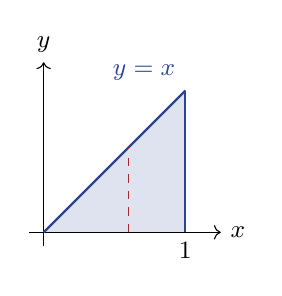
\begin{tikzpicture}[scale=1.8]
\fill[azul!15] (0,0)--(1,0)--(1,1)--cycle;
\draw[->] (-0.1,0)--(1.25,0) node[right]{\small$x$};
\draw[->] (0,-0.1)--(0,1.2) node[above]{\small$y$};
\draw[thick,azul] (0,0)--(1,1) node[above left]{\small$y=x$};
\draw[thick,azul] (1,0)--(1,1);
\draw[rojo,dashed] (0.6,0)--(0.6,0.6);
\node[below] at (1,0){\small1};
\end{tikzpicture}
\end{minipage}
\end{ejemplo}

\begin{ejemplo}[Ejemplo 3 (Clase 18). Cambio de orden para una integral imposible]
$I=\displaystyle\int_0^1\!\!\int_y^1 e^{x^2}\,dx\,dy$. La integral interior no tiene primitiva elemental.
La región es $0\le y\le1$, $y\le x\le1$: es el triángulo $T$ del ejemplo anterior. Como tipo I, $0\le x\le1$, $0\le y\le x$:
\[
I=\int_0^1\!\!\int_0^x e^{x^2}\,dy\,dx=\int_0^1 x\,e^{x^2}\,dx=\Big[\tfrac12e^{x^2}\Big]_0^1=\frac{e-1}2 .
\]
\end{ejemplo}

\begin{ejemplo}[Ejemplo 4 (Clase 18). Marginal de una uniforme en un triángulo]
$(X,Y)$ es uniforme en $T=\{x,y\ge0,\ x+y\le2\}$ (área 2), así que $p=\tfrac12$ en $T$.
El corte vertical en $x$ va de $y=0$ a $y=2-x$:
\[
p_X(x)=\int_0^{2-x}\tfrac12\,dy=\frac{2-x}2\quad(0\le x\le2),\qquad P(X\le\tfrac12)=\int_0^{1/2}\Big(1-\frac x2\Big)dx=\frac7{16}.
\]
La conjunta es constante, pero la marginal no: los cortes largos acumulan más probabilidad.
\end{ejemplo}

\section{Ejercicios}

\ejercicio[Ay 8]{Fubini en rectángulos}
Calcule:
\begin{enumerate}[label=(\alph*),itemsep=0pt]
\item $\iint_R(x+2y)\dA$ con $R=[0,2]\times[0,1]$, en los dos órdenes.
\item $\iint_R x\,e^{xy}\dA$ con $R=[0,1]\times[0,1]$. ¿Qué orden conviene?
\item $\iint_R y\,e^{xy}\dA$ con $R$: $0\le x\le1$, $0\le y\le2$. ¿Qué pasa si intenta el otro orden?
\item $\iint_R\dfrac{x}{1+xy}\dA$ con $R=[0,1]\times[0,1]$.
\end{enumerate}

\ejercicio[Ay 9]{Región entre una parábola y una recta}
Calcule $\iint_D y\dA$, donde $D$ es la región encerrada por la parábola $x=y^2$ y la recta $y=x-2$. Dibuje $D$. ¿Por qué conviene integrar primero en $x$?

\ejercicio[Ay 8 y 9]{Cambio de orden}
Dibuje la región, cambie el orden de integración y calcule:
\[
\text{(a)}\int_0^1\!\!\int_{\sqrt y}^1 e^{x^3}\,dx\,dy\qquad
\text{(b)}\int_0^2\!\!\int_{y/2}^1\cos(x^2)\,dx\,dy\qquad
\text{(c)}\int_0^4\!\!\int_{\sqrt y}^2\sqrt{x^3+1}\,dx\,dy
\]

\ejercicio[Clase 18]{Uniforme en un triángulo}
Un punto se elige al azar (uniforme) en $T=\{0\le x\le y\le1\}$. Encuentre la constante $C$ de la densidad y las marginales $p_X$ y $p_Y$.

\ejercicio[Ay 9]{Densidad no uniforme en un triángulo}
$(X,Y)$ tiene densidad $p(x,y)=C(x+y)$ en $T=\{x\ge0,\ y\ge0,\ x+y\le1\}$ y $0$ fuera. Encuentre $C$, la marginal $p_X$ y $P(X\le\tfrac12)$.

\ejercicio[Ay 8, tipo examen]{Pedidos de delivery}
La ubicación $(X,Y)$ de un pedido en la zona $Q=[0,1]\times[0,1]$ (en km) tiene densidad $p(x,y)=Ce^{x+y}$ en $Q$ y $0$ fuera.
\begin{enumerate}[label=(\alph*),itemsep=0pt]
\item Encuentre $C$. ¿Puede $p(x,y)$ ser mayor que 1? ¿Es un problema?
\item Calcule $P\big((X,Y)\in[0,\tfrac12]^2\big)$ y compárela con un modelo uniforme.
\item Calcule $P(X\le\tfrac12)$. ¿Qué relación tiene con (b)?
\item ¿Qué fracción de los pedidos cae en $[\tfrac12,1]^2$?
\item Calcule $P(X+Y\le1)$ con cortes verticales. ¿Cuánto vale $P(Y\le X)$? (Responda sin integrar.)
\end{enumerate}

\newpage
\section{Soluciones}

\sol{1}
(a) $\int_0^2\int_0^1(x+2y)\,dy\,dx=\int_0^2(x+1)\,dx=4$; en el otro orden, $\int_0^1(2+4y)\,dy=4$.
(b) Primero en $y$: $\int_0^1xe^{xy}\,dy=e^x-1$, luego $\int_0^1(e^x-1)\,dx=e-2\approx0.718$.
(c) Primero en $x$: $\int_0^1ye^{xy}\,dx=e^y-1$, luego $\int_0^2(e^y-1)\,dy=e^2-3\approx4.389$. En el otro orden, $\int_0^2 ye^{xy}\,dy$ requiere integrar por partes y queda una integral en $x$ difícil.
(d) Primero en $y$: $\int_0^1\frac{x}{1+xy}\,dy=\ln(1+x)$, luego $\int_0^1\ln(1+x)\,dx=2\ln2-1\approx0.386$.

\sol{2}
Las curvas se cortan donde $y^2=y+2$, es decir $y=-1$ e $y=2$. Con cortes horizontales, $x$ va de $y^2$ a $y+2$ (siempre las mismas curvas). Con cortes verticales habría que partir $D$ en dos.
\[
\int_{-1}^2\!\!\int_{y^2}^{y+2}y\,dx\,dy=\int_{-1}^2(y^2+2y-y^3)\,dy=\frac94 .
\]

\sol{3}
(a) La región es $0\le y\le x^2$, $0\le x\le1$: $\int_0^1x^2e^{x^3}dx=\frac{e-1}3$.
(b) La región es $0\le y\le2x$, $0\le x\le1$: $\int_0^1 2x\cos(x^2)\,dx=\sin1\approx0.841$.
(c) La región es $0\le y\le x^2$, $0\le x\le2$: $\int_0^2x^2\sqrt{x^3+1}\,dx=\frac29\big[(x^3+1)^{3/2}\big]_0^2=\frac{52}9$.

\sol{4}
El área de $T$ es $\tfrac12$, así que $C=2$. $p_X(x)=\int_x^1 2\,dy=2(1-x)$ y $p_Y(y)=\int_0^y2\,dx=2y$, en $[0,1]$.

\sol{5}
$\int_0^1\int_0^{1-x}(x+y)\,dy\,dx=\frac12\int_0^1(1-x^2)\,dx=\frac13$, así que $C=3$.
$p_X(x)=3\int_0^{1-x}(x+y)\,dy=\frac32(1-x^2)$ para $0\le x\le1$.
$P(X\le\tfrac12)=\frac32\int_0^{1/2}(1-x^2)\,dx=\frac{11}{16}$.

\sol{6}
(a) $\iint_Qe^{x+y}\dA=(e-1)^2$, así que $C=\frac1{(e-1)^2}\approx0.339$. Sí: $p(1,1)=Ce^2\approx2.5>1$. No es problema, porque $p$ es una densidad y no una probabilidad.
(b) $C(e^{1/2}-1)^2=\frac1{(\sqrt e+1)^2}\approx0.143$, contra $0.25$ con el modelo uniforme.
(c) $\frac{\sqrt e-1}{e-1}=\frac1{\sqrt e+1}\approx0.378$. El resultado de (b) es el cuadrado de (c): la densidad es producto $e^x\cdot e^y$ (independencia).
(d) $C(e-\sqrt e)^2=\frac{e}{(\sqrt e+1)^2}\approx0.387$.
(e) $C\int_0^1\int_0^{1-x}e^{x+y}\,dy\,dx=C\int_0^1(e-e^x)\,dx=\frac1{(e-1)^2}\approx0.339$. Por simetría ($p(x,y)=p(y,x)$) y porque la recta $y=x$ tiene probabilidad 0, $P(Y\le X)=\frac12$.

\end{document}
